\titre{Descripteurs de fichier :} Il s'agit d'un nombre entier utilisé ppour identifier un fichier ouvert par un processus. L'OS maintient pour chaque processus une table des descripteurs. \\
Par défaut, 3 descripteurs sont associés à notre programme\\
\begin{tabular}{l|l}
Descripteur & fichier \\ \hline
0 & stdin : lecture du clavier \\ \hline
1 & stdout : écriture dans le terminal \\ \hline
2 & stderr : écriture dans le terminal \\ \hline
\end{tabular} \\
Puis lorsque l'utilisateur réalise la commande open, un nouveau descripteur est créé.\\

\titre{Manipulation :}
\begin{enumerate}
	\item Lecture : read(int fd, void* buf, size\_t count). fd est le descripteur, buf est l'espace mémoire où l'OS va écrire les données lues, et count le nombre d'octets à lire. Retourne le nombre d'octets qui ont réellement été lus, et -1 si erreur.
	\item Ecriture : write(int fd,const void* buf, size\_t count). fd est le descripteur, buf est l'espace mémoire où l'OS va lire les données à écrire dans le fichier, et count le nombre d'octets à écrire. Retourne le nombre d'octets qui ont réellement été écrits, et -1 si erreur.
\end{enumerate}

\titre{Tube : } Fichier virtuel implémentant un canal de communication unidirectionnel. Il a deux extrémités : une en lecture et une en écriture. On manipule les tubes à l'aide de descripteurs de fichiers associés aux extrémités.\\

\titre{Fonctionnement : } 
\begin{enumerate}
	\item Un read effectué sur un tube vide bloque le thread appelant jusqu'à ce qu'un autre thread y écrive des données
	\item Un write effectué sur un tube plein bloque le thread appelant jusqu'à ce qu'un autre thread y lise les données, libérant ainsi de l'espace. 
	\item L'OS garantit que read et write sont atomiques sur les tubes, à condition que la taille des données ne dépasse pas la taille du tube (constante PIPE\_BUF définie dans limits.h) . 
	\item Pour lire ou écrire dans un tube, il faut que les deux extrémités aient été ouvertes. Un tube dont une des extrémités est fermée est dit cassé. 
	\begin{enumerate}
		\item Ecrire dans un tube cassé provoque une erreur
		\item Lire dans un tube vide et cassé ne lit rein et retourne 0.
	\end{enumerate}
\end{enumerate}

\titre{Nommés / non nommés :} Un tube nommé apparait dans le système de fichier, contrairement au non nommé. \\
	\begin{enumerate}
		\item Création de Non nommés :
		\begin{enumerate}
			\item Dans le terminal en séparant deux programmes par le symbole pipe | 
			\item Par la commande int pipe(int df[2]) (df[0] = descripteur du fichier en lecture, df[1] = descripteur du fichier en écriture)
		\end{enumerate}
		\item Création d'un tube nommé
		\begin{enumerate}
			\item mkfifo nomFichier
		\end{enumerate}
	\end{enumerate}
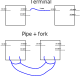
\includegraphics[width=200px]{fig35.pdf} \\
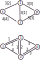
\includegraphics[width=180px]{fig36.pdf} \\
